\documentclass[11pt,fleqn]{book} % Default font size and left-justified equations

\usepackage[top=3cm,bottom=3cm,left=3.2cm,right=3.2cm,headsep=10pt,letterpaper]{geometry} % Page margins
\usepackage{pdfpages}
\usepackage{hyperref}
\usepackage{afterpage}
\usepackage{nopageno}
\usepackage{xcolor} % Required for specifying colors by name
\usepackage{color}
\definecolor{red}{RGB}{231, 76, 60}
\definecolor{cloud}{RGB}{236,240,241}

% Font Settings
\usepackage{helvet}

\usepackage{microtype} % Slightly tweak font spacing for aesthetics
\usepackage[utf8]{inputenc} % Required for including letters with accents
\usepackage[T1]{fontenc} % Use 8-bit encoding that has 256 glyphs

% Bibliography
\usepackage[style=alphabetic,sorting=nyt,sortcites=true,autopunct=true,babel=hyphen,hyperref=true,abbreviate=false,backref=true,backend=biber]{biblatex}
\addbibresource{bibliography.bib} % BibTeX bibliography file
\defbibheading{bibempty}{}


\usepackage{graphicx} % Required for including pictures
\graphicspath{{img/}} % Specifies the directory where pictures are stored
\usepackage{tikz} % Required for drawing custom shapes
\usepackage[english]{babel} % English language/hyphenation

\usepackage{enumitem} % Customize lists
\setlist{nolistsep} % Reduce spacing between bullet points and numbered lists

\usepackage{eso-pic} % Required for specifying an image background in the title page
\usepackage{hyperref}

\begin{document}

%----------------------------------------------------------------------------------------
%	TITLE PAGE
%----------------------------------------------------------------------------------------

\begingroup
\thispagestyle{empty}
\pagecolor{cloud}\afterpage{\nopagecolor}
\centering
\vspace*{3cm}
\par\normalfont\fontsize{35}{35}\sffamily\selectfont
\begin{figure}[h]
    \centering
    
\includegraphics[width=0.4\textwidth]{distributed-systems-red.pdf}
\end{figure}
\vspace*{1cm}
\textbf{Distributed Systems}\\
{\LARGE the source of truth} \\ {\small essential edition}\par
\vspace*{1cm}
\endgroup

%----------------------------------------------------------------------------------------
%	COPYRIGHT PAGE
%----------------------------------------------------------------------------------------

\newpage
~\vfill
\thispagestyle{empty}

\noindent Feel free to contribute at \url{https://github.com/alexprut/distributed-systems}\\ % URL

\noindent \textit{First release, August 2018, version 1.0} % Printing/edition date

%----------------------------------------------------------------------------------------
%	TABLE OF CONTENTS
%----------------------------------------------------------------------------------------
 
\tableofcontents % Print the table of contents itself


\chapter*{Introduction}
\addcontentsline{toc}{chapter}{Introduction}
Both in the libraries and on the internet plenty of resources are available regarding the \textbf{Distributed Systems} topic. All of them are just a better explanation of the same exact source of truth, i.e. academic papers published by the brightest minds in the world. This book is just an ordered collection of all those publications. Below is depicted the order in which you can read the papers. The primary order is based on the citations dependency in the publications, secondary order is based on the year of publication and finally the last criteria is based on the topic dependency.

\vspace*{5mm}

\begin{figure}[h]
\centering
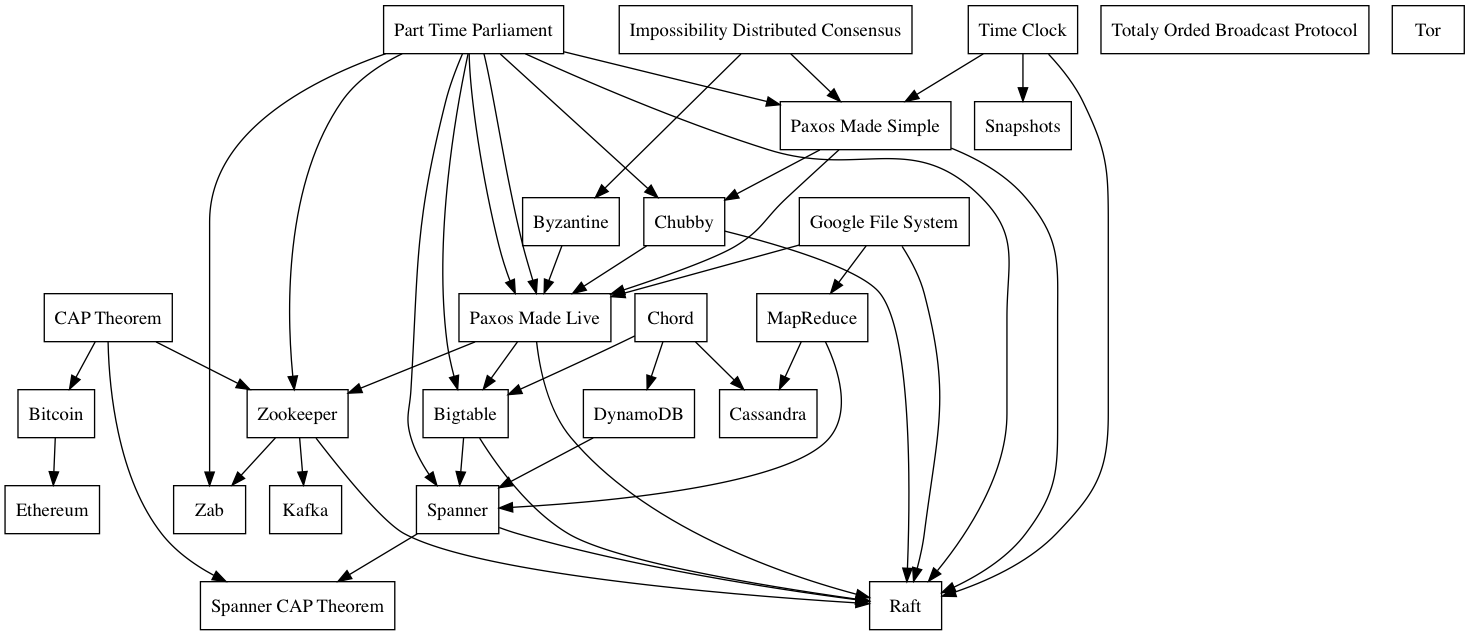
\includegraphics[width=1\textwidth]{dependency}
\end{figure}

\chapter{Time, Clocks, and the Ordering of Events in a Distributed System}
\vspace*{-7mm}
\Large \textbf{Authors}: \\
Leslie Lamport
\newline\newline
\textbf{Publication year}: 1978
\begin{figure}[b]
    \centering
    
\includegraphics[width=0.4\textwidth]{distributed-systems-red.pdf}
\end{figure}
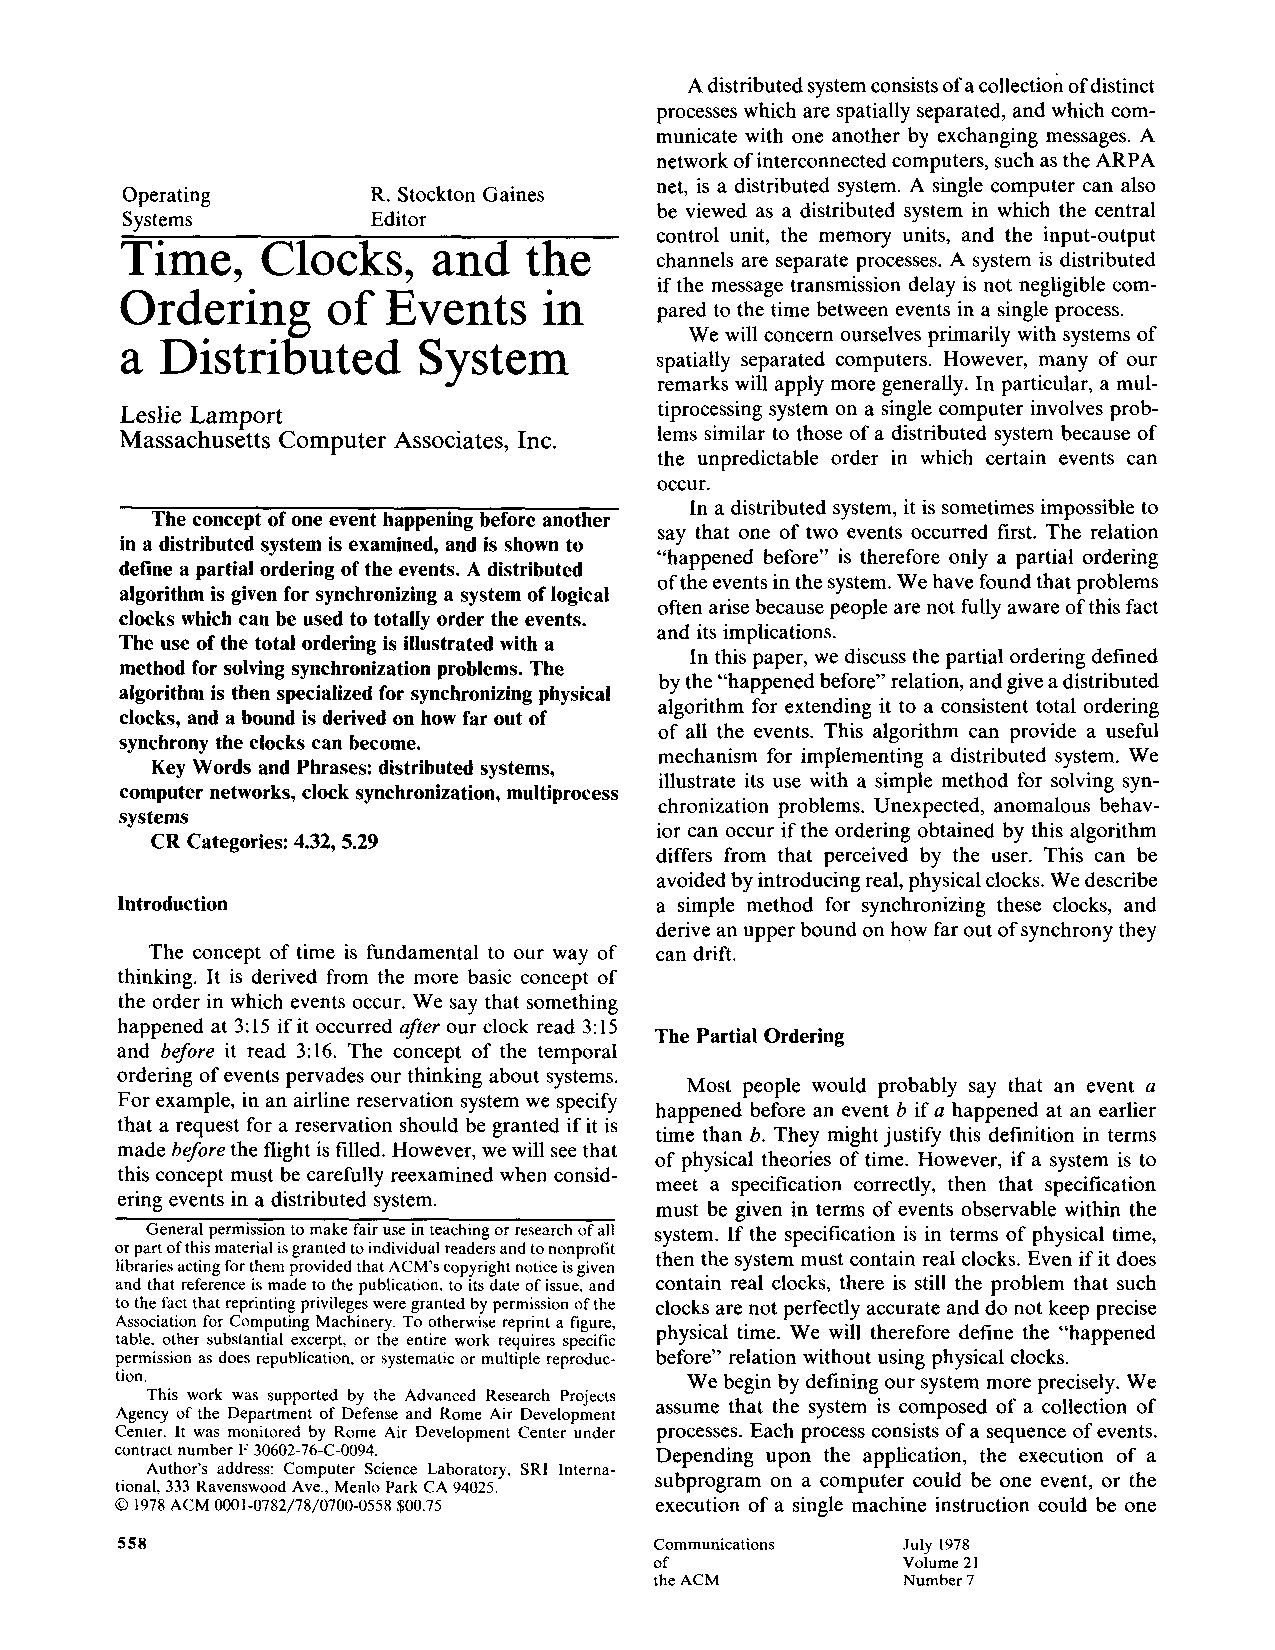
\includepdf[pages=-]{papers/time-clocks.pdf}

\chapter{Distributed Snapshots: Determining Global States of Distributed Systems}
\vspace*{-7mm}
\Large \textbf{Authors}: \\
K. Mani Chandy, Leslie Lamport
\newline\newline
\textbf{Publication year}: 1985
\begin{figure}[b]
    \centering
    
\includegraphics[width=0.4\textwidth]{distributed-systems-red.pdf}
\end{figure}
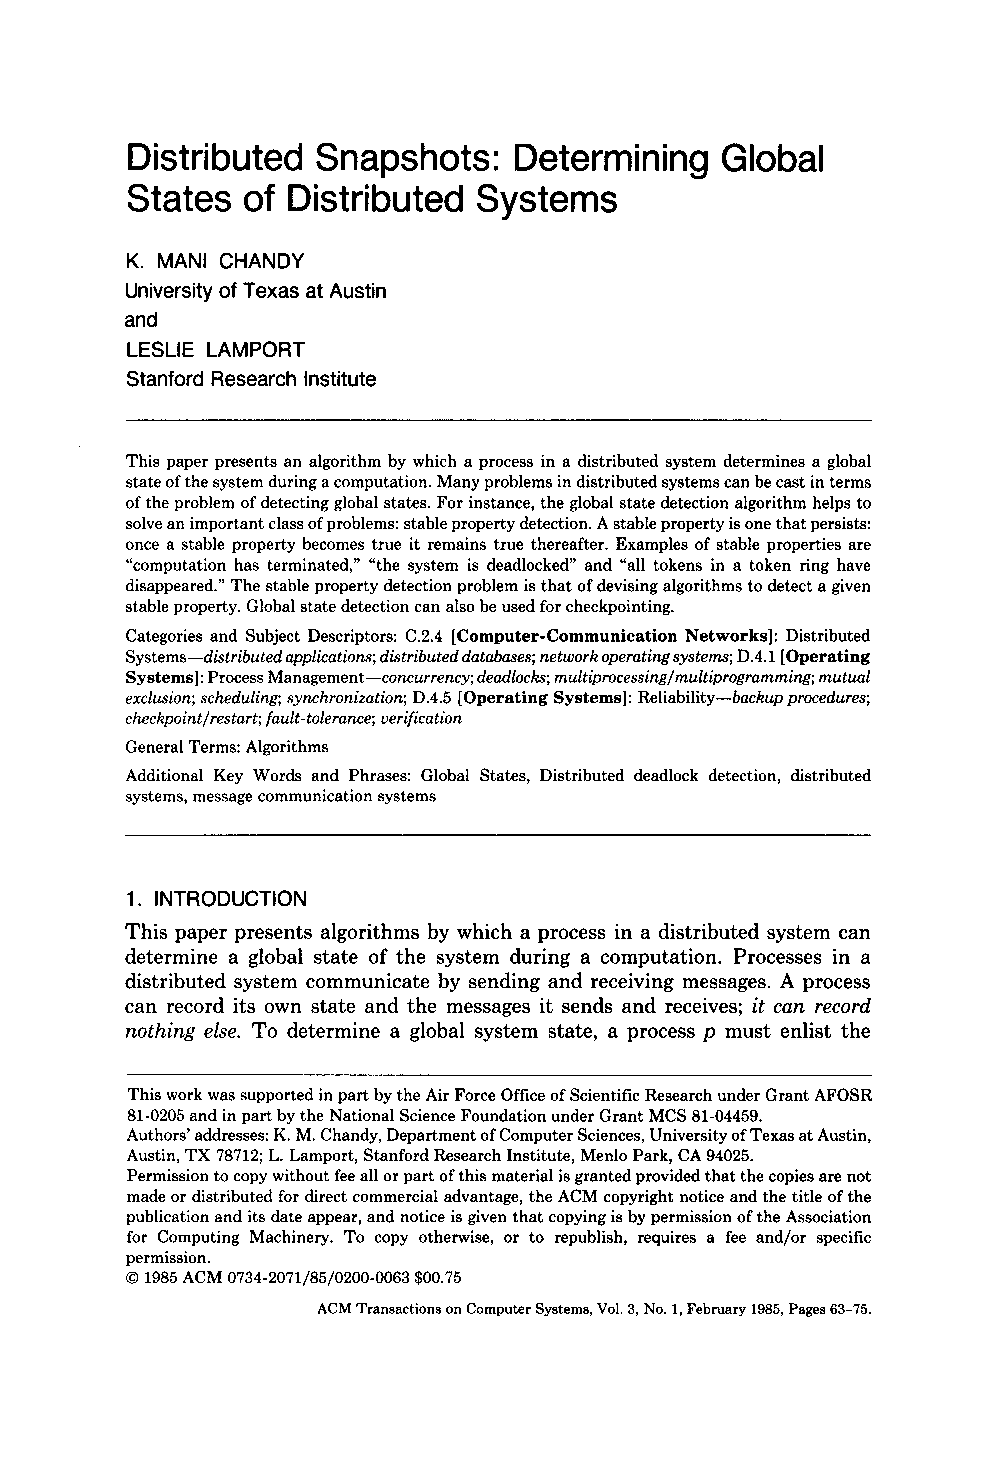
\includepdf[pages=-]{papers/distributed-snapshots.pdf}

\chapter{The Byzantine Generals Problem}
\vspace*{-7mm}
\Large \textbf{Authors}: \\
Leslie Lamport, Robert Shostak, Marshall Pease
\newline\newline
\textbf{Publication year}: 1982
\begin{figure}[b]
    \centering
    
\includegraphics[width=0.4\textwidth]{distributed-systems-triangle-red.pdf}
\end{figure}
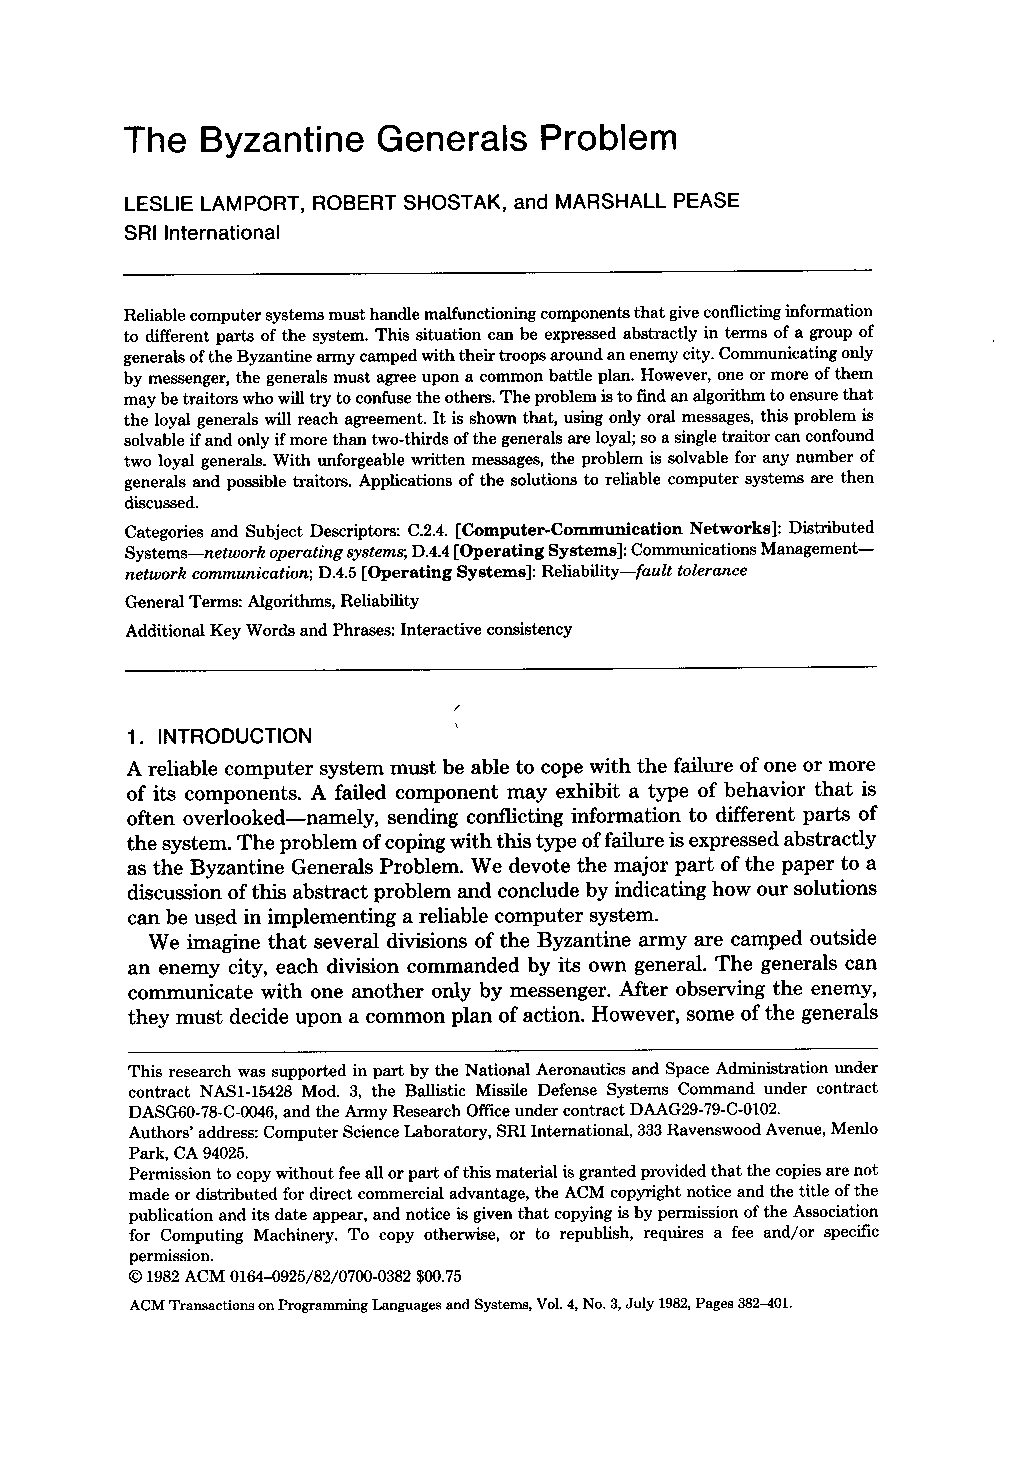
\includepdf[pages=-]{papers/byzantine-generals-problem.pdf}

\chapter{The Part-Time Parliament}
\vspace*{-7mm}
\Large \textbf{Authors}: \\
Leslie Lamport
\newline\newline
\textbf{Publication year}: 1998
\begin{figure}[b]
    \centering
    
\includegraphics[width=0.4\textwidth]{distributed-systems-red.pdf}
\end{figure}
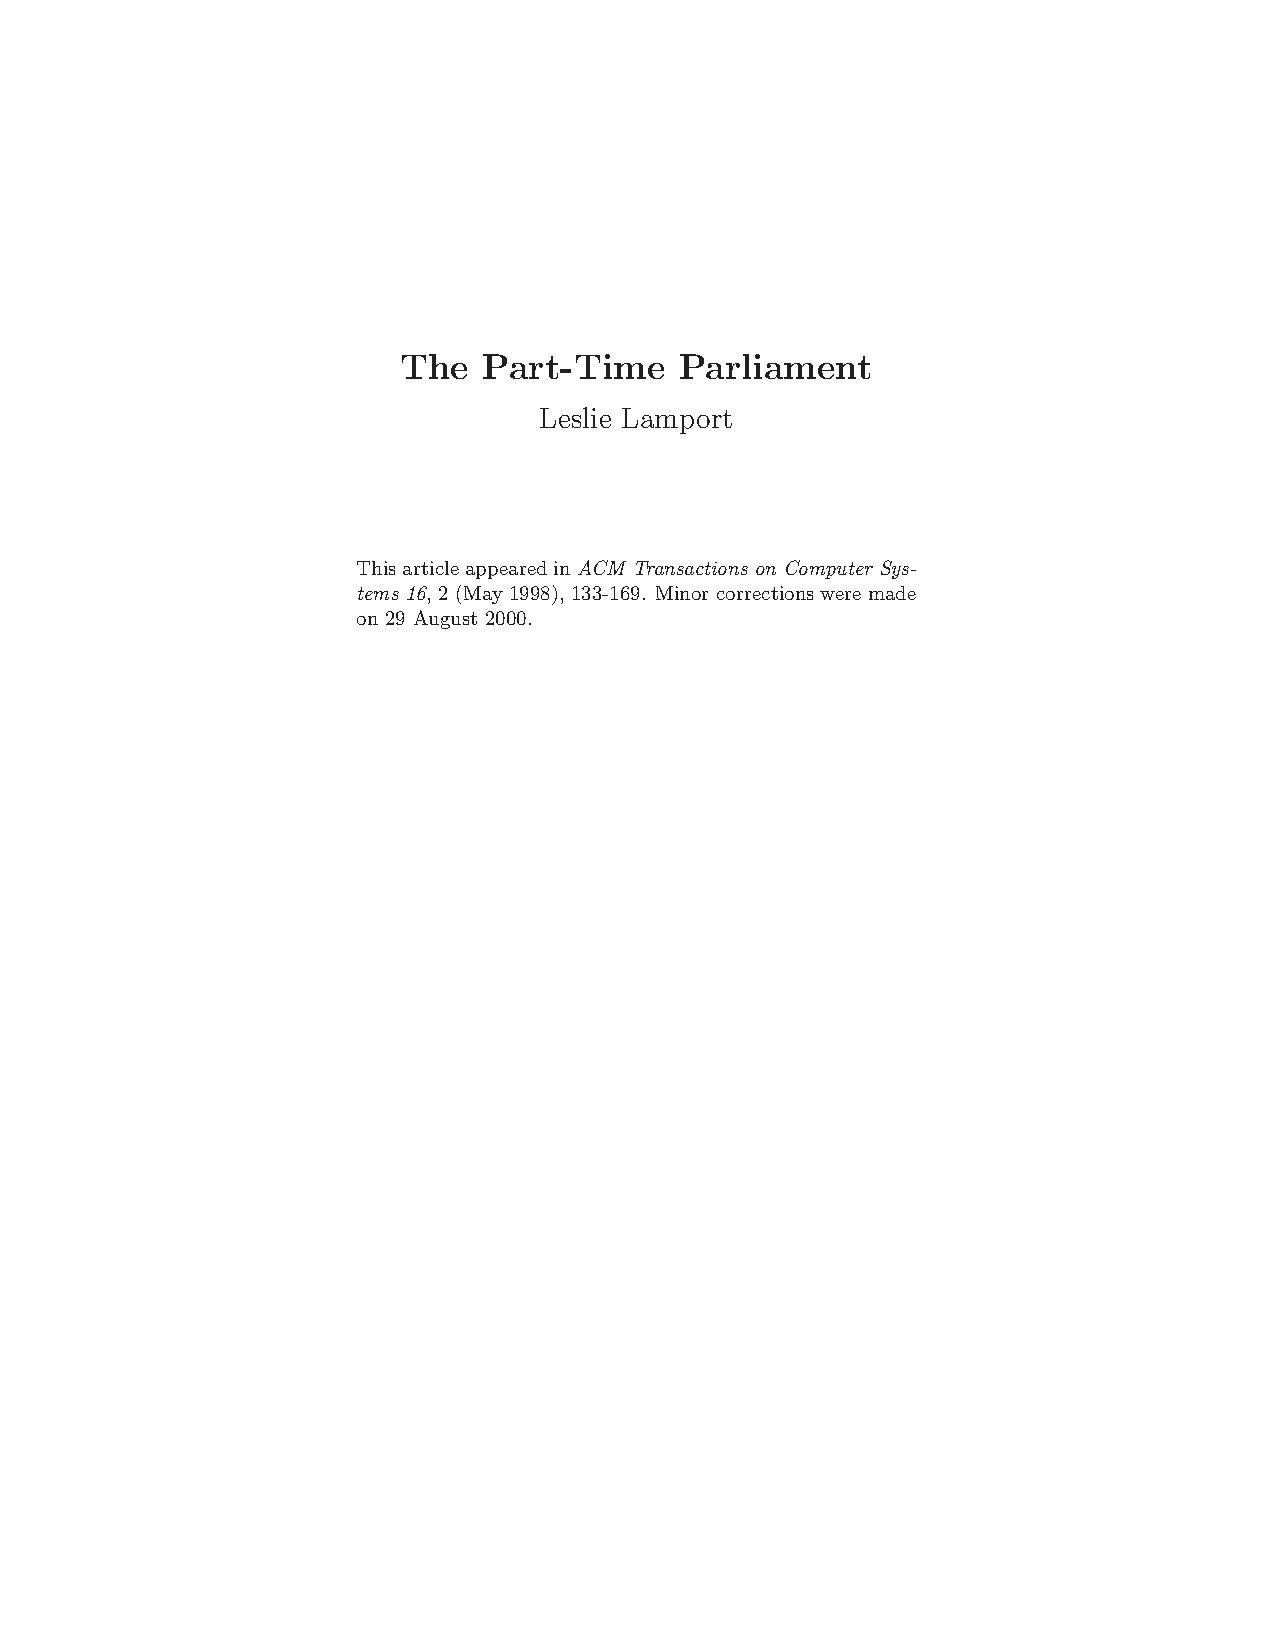
\includepdf[pages=-]{papers/the-part-time-parliament.pdf}

\chapter{Paxos Made Simple}
\vspace*{-7mm}
\Large \textbf{Authors}: \\
Leslie Lamport
\newline\newline
\textbf{Publication year}: 2001
\begin{figure}[b]
    \centering
    
\includegraphics[width=0.4\textwidth]{distributed-systems-red.pdf}
\end{figure}

\includepdf[pages=-]{papers/paxos-made-simple.pdf}

\chapter{Brewer’s Conjecture and the Feasibility of Consistent, Available, Partition-Tolerant Web}
\vspace*{-7mm}
\Large \textbf{Authors}: \\
Seth Gilbert, Nancy Lynch
\newline\newline
\textbf{Publication year}: 2002
\begin{figure}[b]
    \centering
    
\includegraphics[width=0.4\textwidth]{distributed-systems-triangle-red.pdf}
\end{figure}
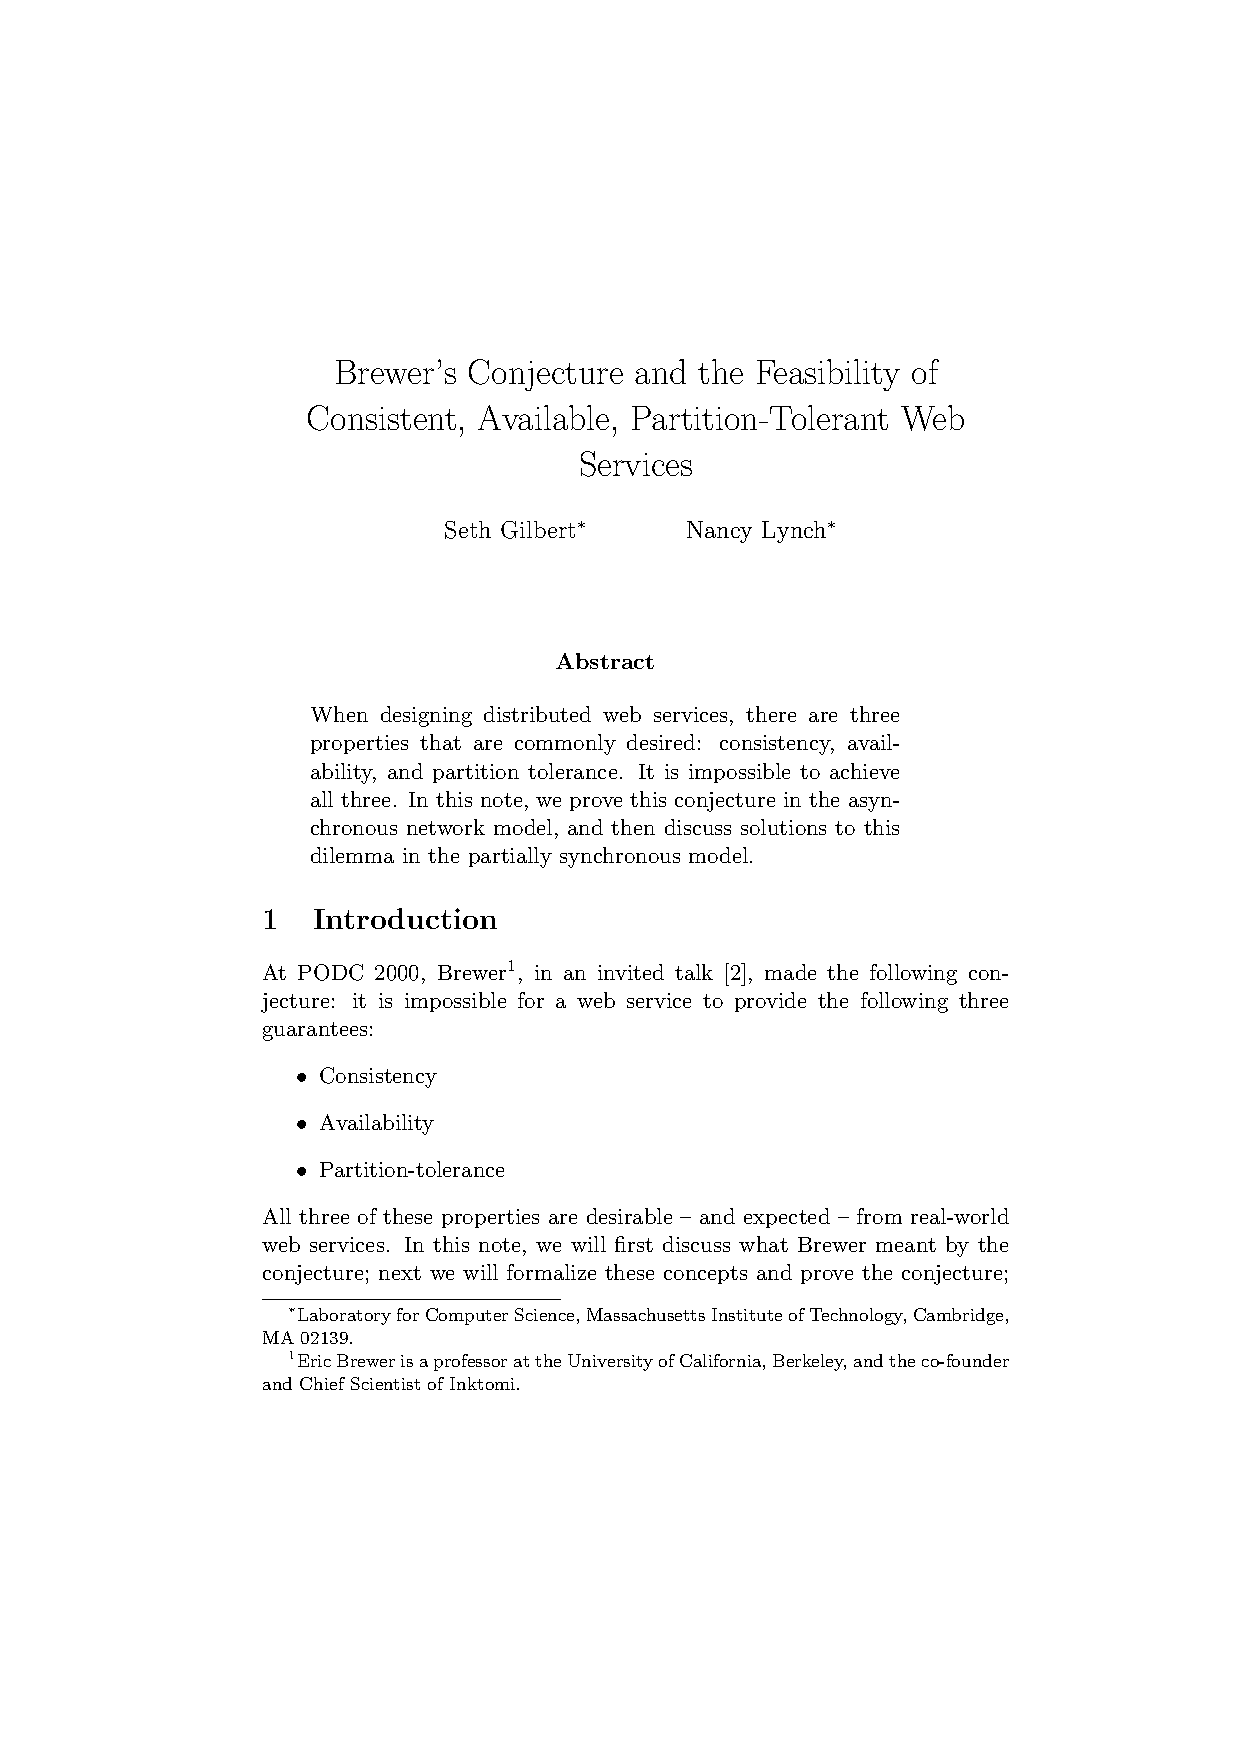
\includepdf[pages=-]{papers/cap-theorem.pdf}

\chapter{MapReduce: Simplified Data Processing on Large Clusters}
\vspace*{-7mm}
\Large \textbf{Authors}: \\
Jeffrey Dean, Sanjay Ghemawat
\newline\newline
\textbf{Publication year}: 2004
\begin{figure}[b]
    \centering
    
\includegraphics[width=0.4\textwidth]{distributed-systems-red.pdf}
\end{figure}
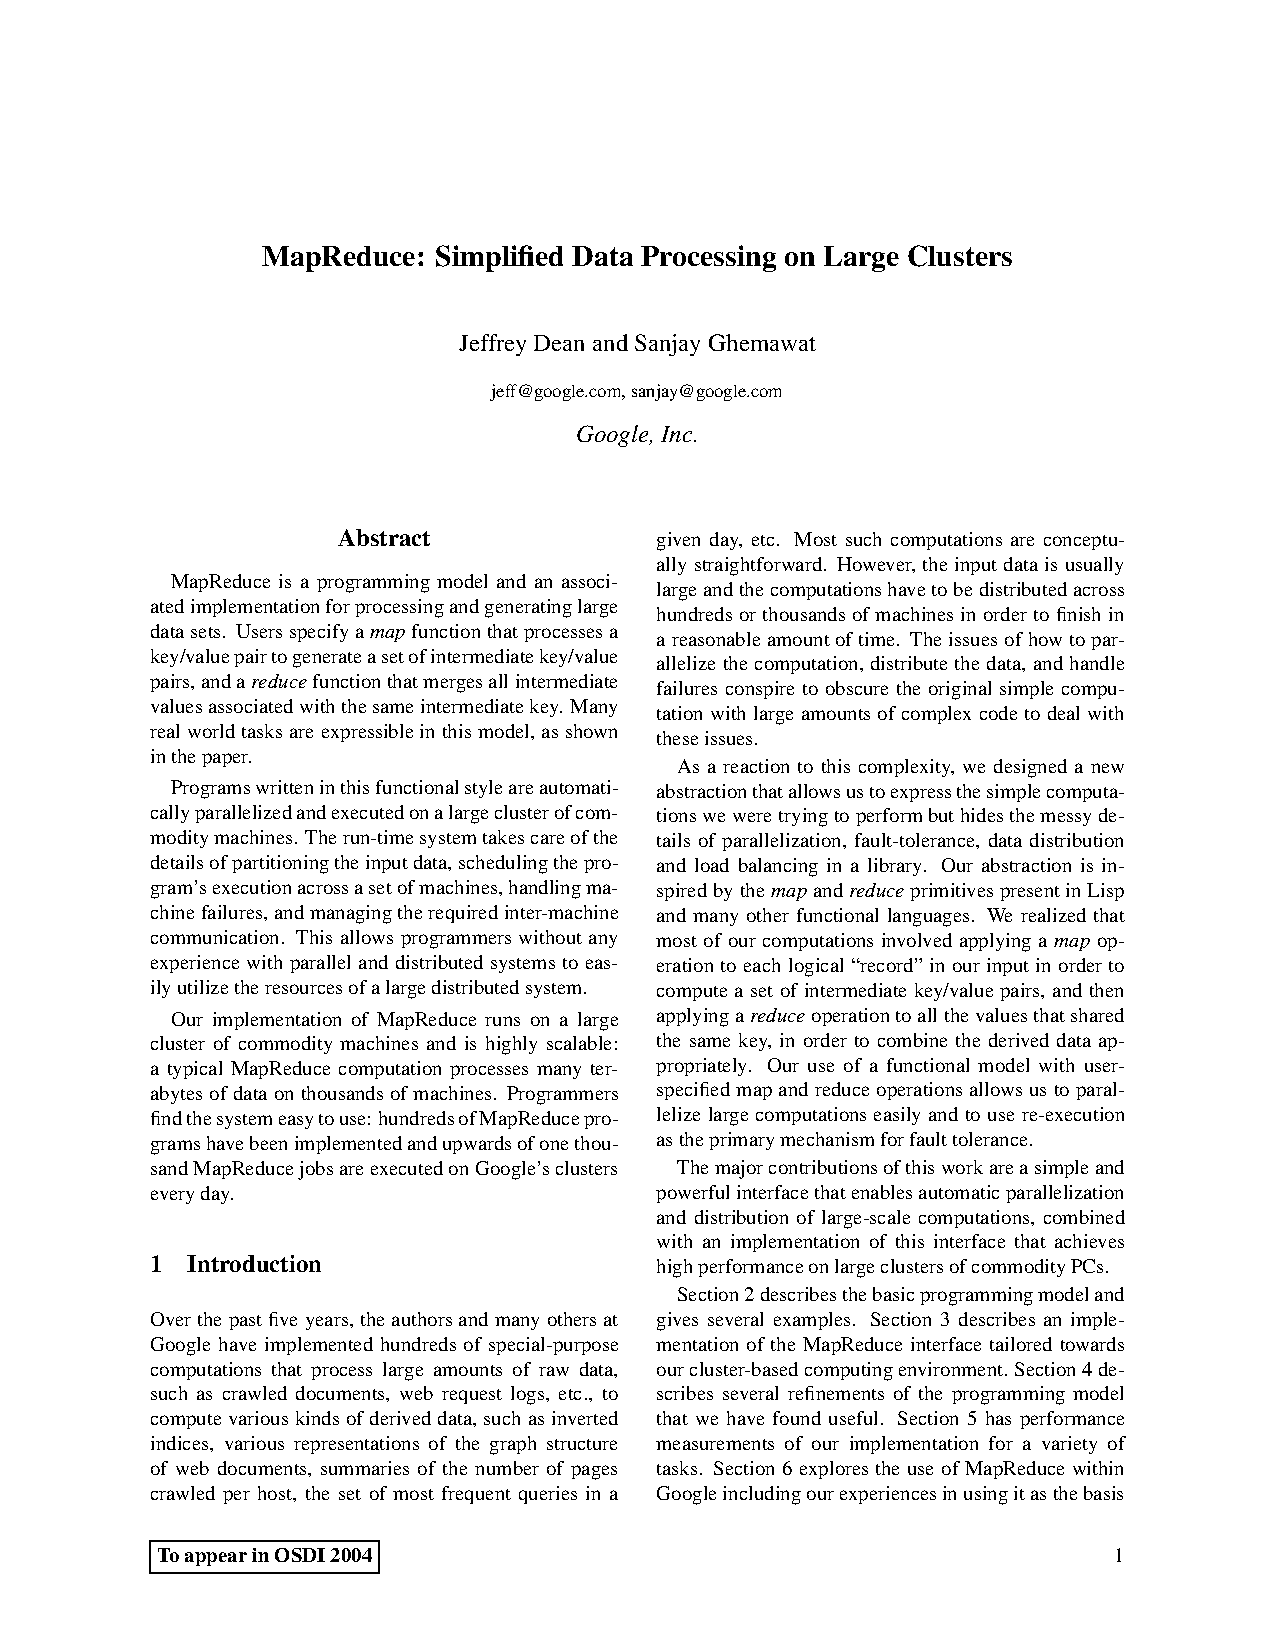
\includepdf[pages=-]{papers/mapreduce.pdf}

\chapter{Paxos Made Live - An Engineering Perspective}
\vspace*{-7mm}
\Large \textbf{Authors}: \\
Tushar Chandra, Robert Griesemer, Joshua Redstone
\newline\newline
\textbf{Publication year}: 2007
\begin{figure}[b]
    \centering
    
\includegraphics[width=0.4\textwidth]{distributed-systems-red.pdf}
\end{figure}
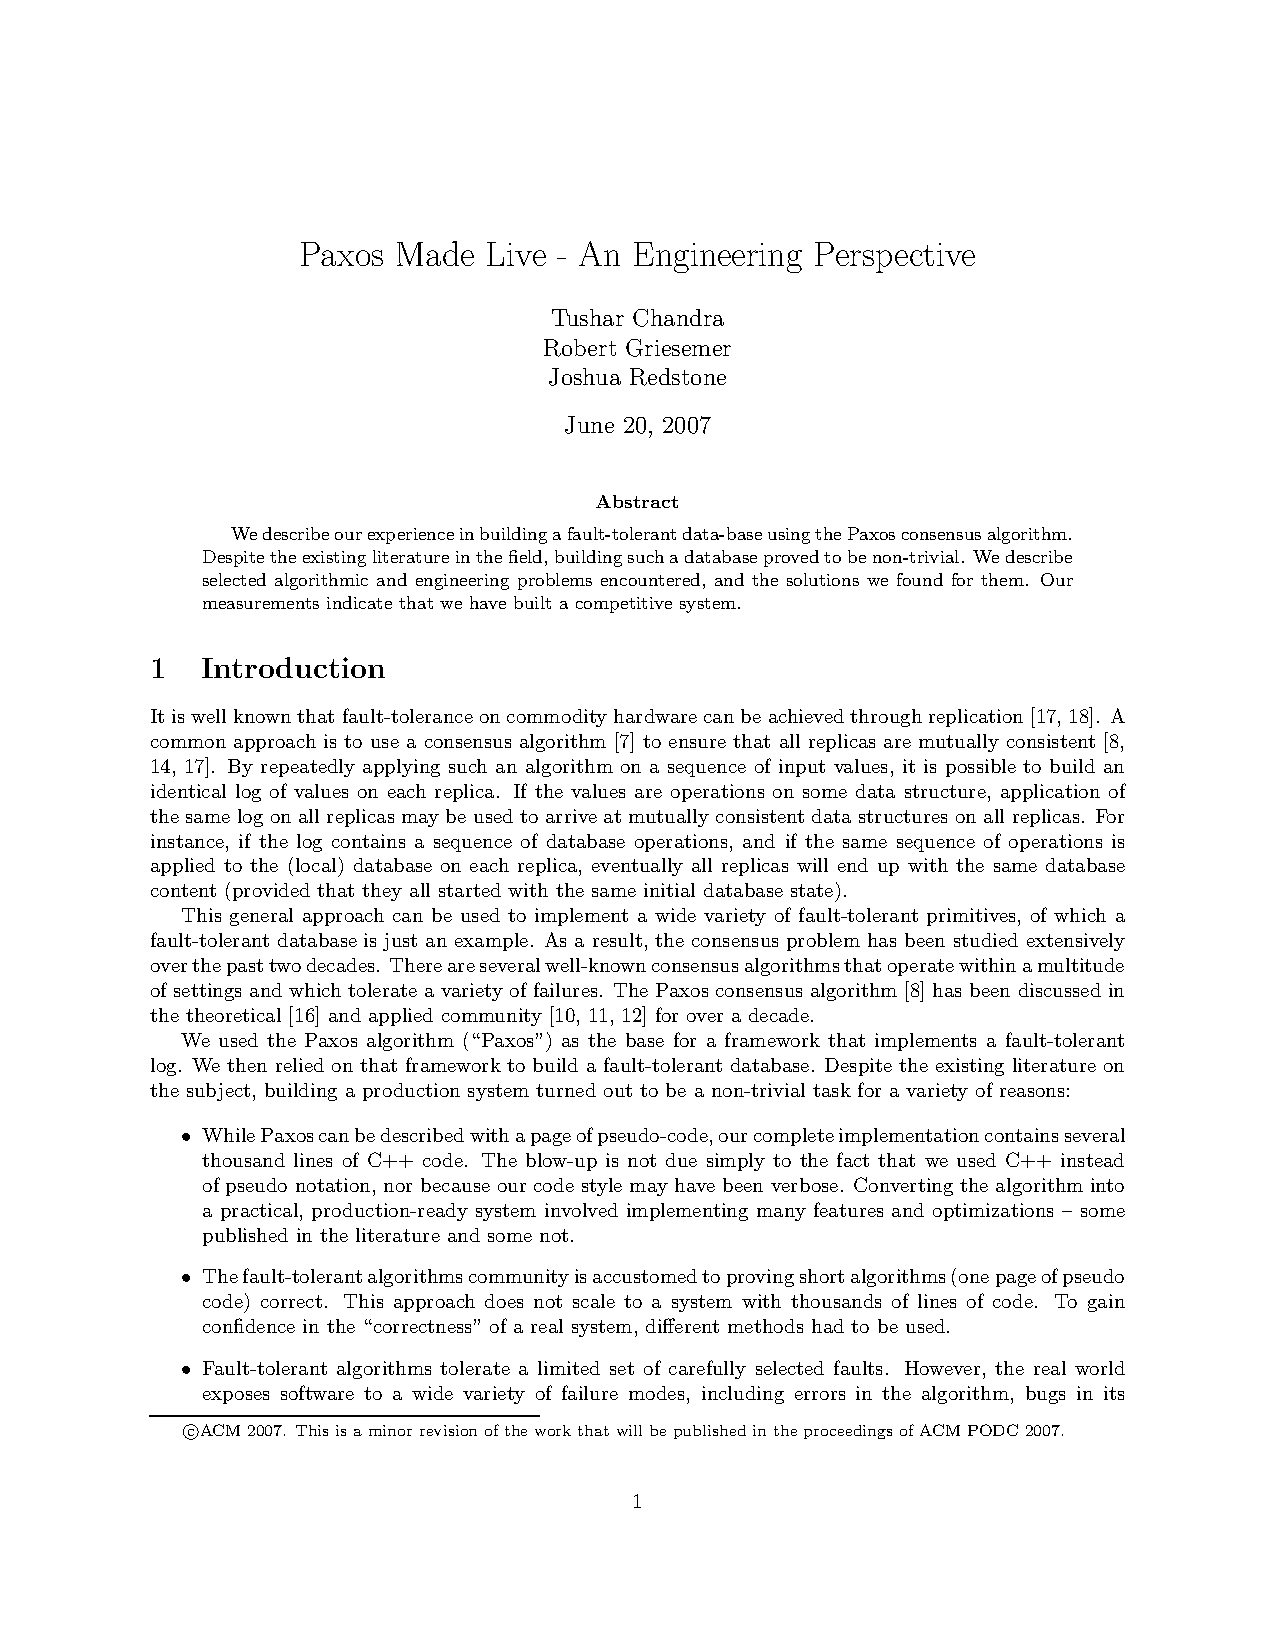
\includepdf[pages=-]{papers/paxos-made-live.pdf}

\chapter{Bitcoin: A Peer-to-Peer Electronic Cash System}
\vspace*{-7mm}
\Large \textbf{Authors}: \\
Satoshi Nakamoto
\newline\newline
\textbf{Publication year}: 2008
\begin{figure}[b]
    \centering
    
\includegraphics[width=0.4\textwidth]{distributed-systems-red.pdf}
\end{figure}
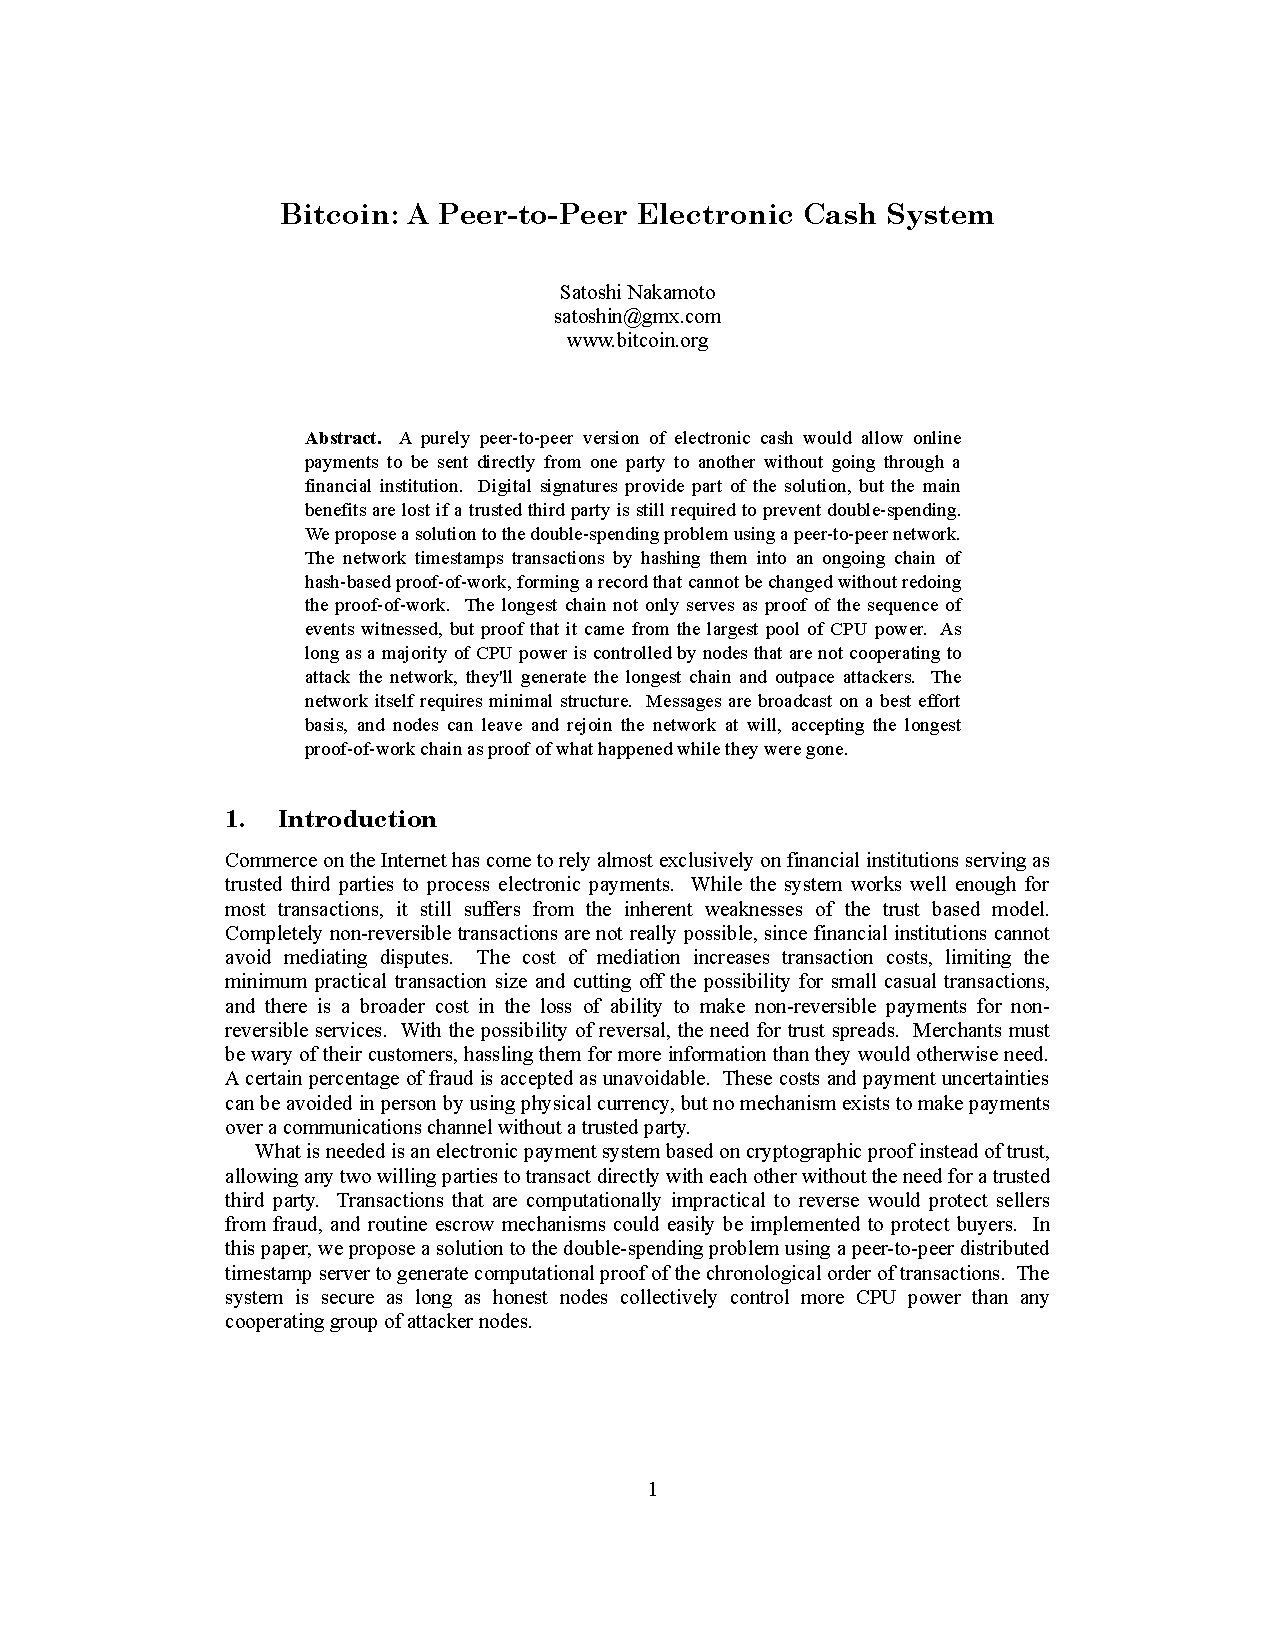
\includepdf[pages=-]{papers/bitcoin.pdf}

\pagecolor{red}\afterpage{}
\newpage\null\thispagestyle{empty}\newpage

\end{document}